\documentclass[tikz,border=2pt]{standalone}
\usepackage{tikz}
\usetikzlibrary{arrows.meta, bending,calc,decorations.markings}

\tikzset{
  midarrow/.style={
    postaction={decorate,
      decoration={
        markings,
        mark=at position 0.5 with {\arrow{Stealth}}
      }
    }
  }
}
\begin{document}
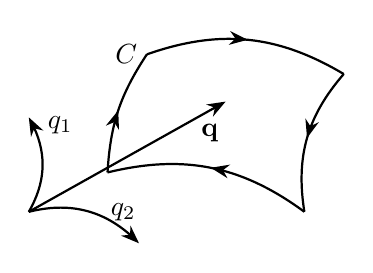
\begin{tikzpicture}[>=Stealth]

% --- Coordinate System Axes (Bottom Left) ---
\coordinate (O) at (0,0);
\draw[->, thick, bend right=30] (O) to (0,1.2);
\node at (0.4,1.1) {$q_1$};
\draw[->, thick, bend left=30] (O) to (1.4,-0.4);
\node at (1.2,0) {$q_2$};


% --- Volume Element ---
\coordinate (A1) at (1,0.5);
\coordinate (A2) at (1.5,2);
\coordinate (A3) at (4,1.75);
\coordinate (A4) at (3.5,0);

\draw[thick, midarrow] (A1) to[bend left=15] (A2);
  \draw[thick, midarrow] (A2) to[bend left=25] (A3);
  \draw[thick, midarrow] (A3) to[bend left=-25] (A4); % Adjusted bend to keep flow
  \draw[thick, midarrow] (A4) to[bend right=25] (A1);

% --- Vectors and Lines ---
\draw[->, thick] (O) -- (2.5, 1.4);
\node at (2.3,1){$\mathbf{q}$};


% Labels 
\node[left] at (1.5, 2.) {$C$};


\end{tikzpicture}
\end{document}